\chapter{Equilibrio: cuando nada se mueve}\label{ch:g2:balance-equilibrium}

Un balancín se queda horizontal con un niño en cada punta. Una torre
de piezas se sostiene --- una pieza más y se derrumba. Una acróbata
camina por una cuerda más fina que su zapato. Los tres están jugando
al mismo juego profundo: el juego del \omterm{def:g2:balance-equilibrium:equilibrium}{equilibrio}, donde las \omterm{def:g2:pushes-and-pulls:force}{fuerzas} se
anulan y nada se mueve.

\section{Estar quieto es un equilibrio}

\begin{definition}[El equilibrio]\label{def:g2:balance-equilibrium:equilibrium}
Una cosa está en \emph{equilibrio}\index{equilibrio} --- también
decimos que está \emph{equilibrada}\index{equilibrada} --- cuando los
empujones y los tirones que recibe se anulan entre sí, de modo que se
queda exactamente como está. La cinta del juego de tirar de la cuerda
quieta entre dos equipos tremendos: equilibrio. No es un mundo sin
\omterm{def:g2:pushes-and-pulls:force}{fuerzas}, sino un mundo donde las \omterm{def:g2:pushes-and-pulls:force}{fuerzas} han quedado en tablas.
\end{definition}

\begin{example}[El libro sobre la mesa]\label{ex:g2:balance-equilibrium:book}
Un libro está sobre la mesa, completamente quieto. ¿Aburrido? Míralo
más de cerca con los ojos del capítulo anterior. La Tierra tira del
libro hacia abajo --- entonces, ¿por qué no se cae? Porque la mesa lo
empuja hacia \emph{arriba} exactamente con la misma intensidad con la
que la Tierra tira hacia abajo. Dos flechas iguales y opuestas: unas
tablas. Quita la mesa y las tablas se rompen: el libro se va abajo.
\end{example}

\begin{omfigure}
\begin{tikzpicture}[scale=0.85]
  \draw[thick] (0.4,1.2) -- (5.6,1.2);
  \draw[thick] (0.9,1.2) -- (0.9,0) (5.1,1.2) -- (5.1,0);
  \draw[thick, fill=omMeth, fill opacity=0.4]
    (2.2,1.2) rectangle (3.8,1.75);
  \node[font=\small] at (3.0,1.47) {libro};
  \draw[-Stealth, very thick, omDef] (3.0,1.1) -- (3.0,0.25);
  \node[right, font=\small, omDef] at (3.15,0.6)
    {la Tierra tira hacia abajo};
  \draw[-Stealth, very thick, omThm] (3.0,1.85) -- (3.0,2.7);
  \node[right, font=\small, omThm] at (3.15,2.4)
    {la mesa empuja hacia arriba};
\end{tikzpicture}

{\small Lo más quieto de la habitación son unas tablas perfectas: dos
flechas iguales en sentidos contrarios. \omterm{def:g2:balance-equilibrium:equilibrium}{Equilibrio}.}
\end{omfigure}

\begin{remark}[Quieto no significa sin fuerzas]\label{rem:g2:balance-equilibrium:notfree}
Antes de este capítulo, ``al libro no le está pasando nada'' parecía
evidente. Ahora ya sabes más: sobre él actúan dos \omterm{def:g2:pushes-and-pulls:force}{fuerzas} en cada
instante. A tu alrededor, las sillas, las lámparas, las casas y las
montañas se sostienen gracias a silenciosas tablas de tirones y
empujones. La quietud no es vacío --- es \omterm{def:g2:balance-equilibrium:equilibrium}{equilibrio}.
\end{remark}

\section{El balancín}

\begin{example}[Unas tablas en el patio]\label{ex:g2:balance-equilibrium:seesaw}
Dos amigos de más o menos el mismo tamaño se sientan en las dos puntas
de un balancín: se queda horizontal --- tablas. Ahora se sienta papá
en una punta: él se va abajo y el niño sale disparado hacia arriba.
Para jugar limpio, papá se desliza \emph{hacia el centro}: cuanto más
cerca se sienta del punto de apoyo, menos aprieta su lado --- hasta
que, justo en el sitio adecuado, el balancín vuelve a quedarse
horizontal. Un peso grande cerca del centro puede empatar con un peso
pequeño bien alejado.
\end{example}

\begin{omfigure}
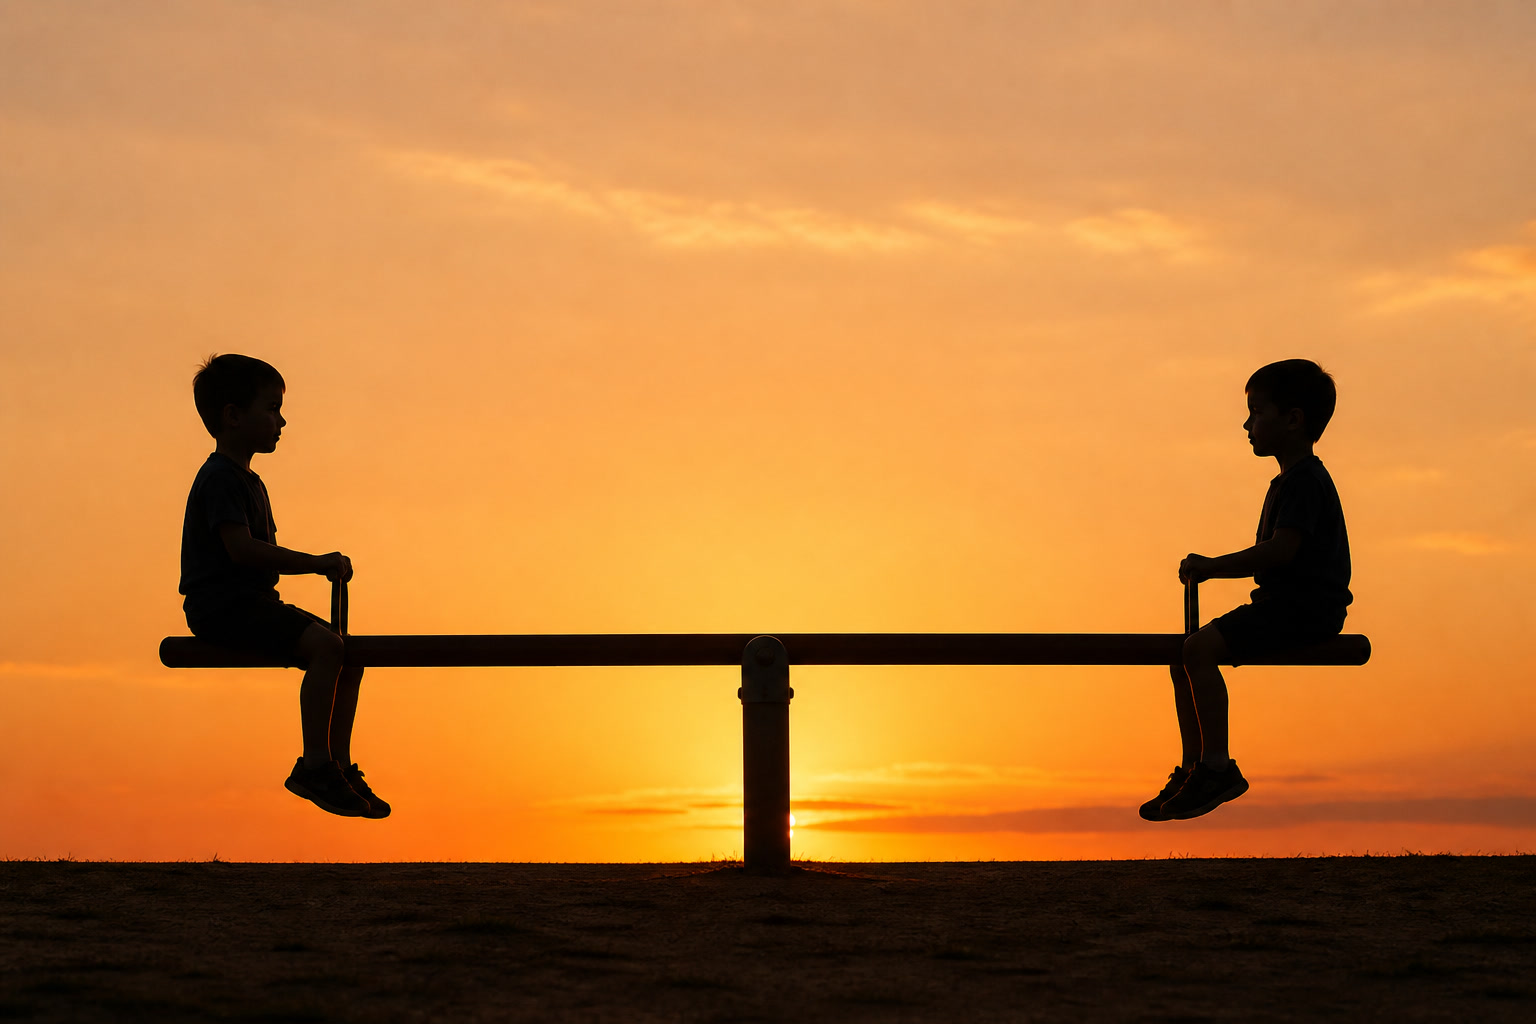
\includegraphics[width=0.58\linewidth]{images/book1/ai/g2-balance-seesaw.jpg}

{\small Unas tablas perfectas en el patio: dos jinetes del mismo tamaño, a la misma distancia --- y el balancín se queda horizontal.}
\end{omfigure}

\begin{proposition}[La regla del balancín]\label{prop:g2:balance-equilibrium:rule}
Pesos iguales a distancias iguales del punto de apoyo se equilibran.
Un jinete más pesado vuelca el balancín --- salvo que el jinete
pesado se acerque al punto de apoyo o el ligero se aleje. Cuentan
tanto el peso \emph{como} la distancia.
\end{proposition}

\begin{omfigure}
\begin{tikzpicture}[scale=0.85]
  \draw[thick, fill=omExo, fill opacity=0.3]
    (2.6,0) -- (3.0,0.75) -- (2.2,0.75) -- cycle;
  \draw[very thick] (0.2,0.8) -- (5.0,0.8);
  \fill[omDef] (0.55,1.1) circle (0.26);
  \fill[omDef] (4.65,1.1) circle (0.26);
  \node[below, font=\small, align=center] at (2.6,-0.25)
    {pesos iguales, distancias iguales:\\horizontal};
  \draw[thick, fill=omExo, fill opacity=0.3]
    (8.9,0) -- (9.3,0.75) -- (8.5,0.75) -- cycle;
  \draw[very thick] (6.5,0.8) -- (11.3,0.8);
  \fill[omThm] (9.9,1.15) circle (0.4);
  \fill[omDef] (6.85,1.1) circle (0.26);
  \node[below, font=\small, align=center] at (8.9,-0.25)
    {el jinete pesado se sienta cerca:\\horizontal otra vez};
\end{tikzpicture}

{\small Dos caminos hacia las tablas: pesos iguales a distancias
iguales --- o un jinete pesado cerca del punto de apoyo contra un
jinete ligero bien alejado.}
\end{omfigure}

\begin{remark}[Una promesa]\label{rem:g2:balance-equilibrium:promise}
¿Y hasta dónde tiene que deslizarse papá, exactamente? En el balancín
se esconde una regla preciosa y precisa --- con números de verdad
dentro. Te espera el año que viene, en el capítulo de las palancas y
las balanzas; los juegos de balancín de hoy son su entrenamiento
perfecto.
\end{remark}

\section{Volcar y el punto de equilibrio}

\begin{example}[La torre que se inclinó demasiado]\label{ex:g2:balance-equilibrium:tower}
Construye una torre de piezas, cada una asomando un poco más que la de
debajo. Se sostiene, se sostiene\dots\ y de pronto se derrumba. Una
cosa inclinada vuelca cuando se sale \emph{demasiado} de su propia
base. Por eso una pirámide de piezas con la base ancha es dificilísima
de tirar, mientras que una columna alta y sola se cae con un soplido:
los pies anchos hacen torres firmes.
\end{example}

\begin{definition}[El punto de equilibrio]\label{def:g2:balance-equilibrium:point}
El \emph{punto de equilibrio}\index{punto de equilibrio} de un objeto
es el sitio especial por el que se puede sostener horizontal --- como
si todo su peso se hubiera juntado allí. Una regla lleva su punto de
\omterm{def:g2:balance-equilibrium:equilibrium}{equilibrio} en el centro; un martillo lo esconde cerca de su cabeza
pesada. Sujetado justo por debajo de su punto de \omterm{def:g2:balance-equilibrium:equilibrium}{equilibrio},
cualquier objeto descansa horizontal sobre un dedo.
\end{definition}

\begin{method}[Encontrar el punto de equilibrio]\label{met:g2:balance-equilibrium:find}
Para encontrar el \omterm{def:g2:balance-equilibrium:point}{punto de equilibrio} de una regla, una escoba o una
cuchara de madera:
\begin{enumerate}
  \item apóyalo sobre los dos dedos índice estirados, uno cerca de
        cada extremo;
  \item desliza los dedos despacio el uno hacia el otro;
  \item se encontrarán --- siempre con el objeto todavía
        equilibrado --- en un solo sitio: el \omterm{def:g2:balance-equilibrium:point}{punto de equilibrio}.
\end{enumerate}
Pruébalo con la escoba: los dedos se encuentran lejos del centro, del
lado del cepillo pesado. Al \omterm{def:g2:balance-equilibrium:point}{punto de equilibrio} le encanta el lado
pesado.
\end{method}

\begin{omfigure}
\begin{tikzpicture}[scale=0.85]
  \draw[thick, fill=omMeth, fill opacity=0.4]
    (0.3,1.5) rectangle (6.3,1.78);
  \draw[thick] (1.1,0.6) -- (1.1,1.45) (5.5,0.6) -- (5.5,1.45);
  \draw[-Stealth, omExo, thick] (1.45,0.9) -- (2.6,0.9);
  \draw[-Stealth, omExo, thick] (5.15,0.9) -- (4.0,0.9);
  \node[below, font=\small] at (3.3,0.45)
    {desliza los dos dedos hacia dentro\dots};
  \draw[thick, fill=omMeth, fill opacity=0.4]
    (7.6,1.5) rectangle (11.6,1.78);
  \draw[thick] (9.6,0.6) -- (9.6,1.45);
  \fill[omThm] (9.6,1.92) circle (2.2pt);
  \node[below, font=\small] at (9.6,0.45)
    {\dots{}se encuentran bajo el punto de equilibrio};
\end{tikzpicture}

{\small El truco de los dos dedos: los dedos que se deslizan acaban
siempre justo debajo del \omterm{def:g2:balance-equilibrium:point}{punto de equilibrio}.}
\end{omfigure}

\begin{example}[La pértiga de la acróbata]\label{ex:g2:balance-equilibrium:acrobat}
¿Por qué lleva la funambulista esa pértiga larga y caída por las
puntas? Es su ayudante de \omterm{def:g2:balance-equilibrium:equilibrium}{equilibrio}: cuando empieza a inclinarse
hacia un lado, la pértiga larga hace que la caída sea lenta y
perezosa en vez de rápida, y le da tiempo a volver a colocarse sobre
la cuerda. Tú usas el mismo truco con los brazos desnudos cuando
caminas por un bordillo --- brazos abiertos, bamboleo más lento,
\omterm{def:g2:balance-equilibrium:equilibrium}{equilibrio} salvado.
\end{example}

\section{Ejercicios}

\begin{exercise}[$\star$]\label{exo:g2:balance-equilibrium:1}
Una lámpara está quieta sobre el escritorio. Nombra las dos \omterm{def:g2:pushes-and-pulls:force}{fuerzas}
que actúan sobre ella y di por qué no se mueve.
\end{exercise}

\begin{exercise}[$\star$]\label{exo:g2:balance-equilibrium:2}
En el juego de tirar de la cuerda, ¿cuándo está la cinta en
\omterm{def:g2:balance-equilibrium:equilibrium}{equilibrio}? ¿Qué rompe las tablas?
\end{exercise}

\begin{exercise}[$\star$]\label{exo:g2:balance-equilibrium:3}
Dos gemelas iguales se sientan en un balancín a la misma distancia.
¿Qué hace el balancín? Una de ellas se desliza hacia atrás, más lejos
del punto de apoyo --- ¿qué lado baja ahora?
\end{exercise}

\begin{exercise}[$\star$]\label{exo:g2:balance-equilibrium:4}
Papá pesa mucho más que Lina y, sin embargo, su balancín se queda
horizontal. ¿Dónde tiene que estar sentado papá? Enuncia la regla que
salva el juego.
\end{exercise}

\begin{exercise}[$\star$]\label{exo:g2:balance-equilibrium:5}
¿Dónde está el \omterm{def:g2:balance-equilibrium:point}{punto de equilibrio} de una regla? ¿Y el de un martillo:
hacia la punta del mango o hacia la cabeza pesada? ¿Cómo podrías
comprobarlo con un solo dedo?
\end{exercise}

\begin{exercise}[$\star$]\label{exo:g2:balance-equilibrium:6}
Haz el truco de los dos dedos del
\cref{met:g2:balance-equilibrium:find} con una escoba. ¿De qué lado se
encuentran tus dedos y qué te dice eso?
\end{exercise}

\begin{exercise}[$\star$]\label{exo:g2:balance-equilibrium:7}
¿Qué se sostiene con más firmeza y por qué: una pirámide de piezas con
la base ancha o una torre de una pieza de ancho y la misma altura?
\end{exercise}

\begin{exercise}[$\star$]\label{exo:g2:balance-equilibrium:8}
¿Por qué lleva una pértiga larga quien camina por la cuerda floja?
¿Qué haces tú con los brazos cuando caminas por un bordillo y por qué
ayuda?
\end{exercise}

\begin{exercise}[$\star$]\label{exo:g2:balance-equilibrium:9}
Ponte de pie con el hombro derecho y el pie derecho pegados a una
pared e intenta levantar el pie izquierdo. ¡No puedes, sin caerte!
Explícalo con la torre del \cref{ex:g2:balance-equilibrium:tower}: ¿qué
tendría que hacer tu cuerpo para sostenerse sobre el pie derecho y qué
le prohíbe la pared?
\end{exercise}

\begin{exercise}[$\star\star$]\label{exo:g2:balance-equilibrium:10}
Una grúa de obra levanta cargas pesadas con su largo brazo delantero
--- y aun así no vuelca. Sobre su corto brazo trasero hay enormes
bloques de hormigón. Explica la grúa con la regla del balancín de la
\cref{prop:g2:balance-equilibrium:rule}: ¿cuáles son los dos jinetes y
por qué es corto el brazo trasero?
\end{exercise}
